\documentclass{article}
\usepackage{hyperref}
\usepackage{multirow}
\usepackage{array}
\usepackage{xeCJK}
\usepackage{listings}
\lstset{
	basicstyle = \small\ttfamily,
	breaklines = true,
	frame = single,
	language = python,
	tabsize = 2,
	showspaces = false,
	showstringspaces = false,
	breakindent =1.1em,
}
\setCJKmainfont[BoldFont={Microsoft YaHei}, ItalicFont={KaiTi}]{SimSun}
\setCJKsansfont{BoldFont=Microsoft YaHei}
\setCJKmonofont{KaiTi}

\title{基于LDA的学术会议主题发现}
\author{游沛杰 13307130325}
\date{2016-1-8}
\begin{document}
\maketitle
\tableofcontents
\newpage

\section{选题介绍}

本次项目我们实现了一个论文主题发现系统,通过对近年学术会议论文使用LDA提取主题并分析,从而发现相关领域的研究进展。

之前考虑过的其他想法如下:
\begin{enumerate}
	\item	研究小学语文的连词成句*,让计算机参加小升初?
	\item	可视化关键词在文章中出现的位置,进一步分析各种词语的重要性来研究人的阅读习惯。
	\item	“自动(好吃的)菜名生成器”以及相关分析,进一步通过菜名和食谱文章用词来描述不同研究八大菜系特点并在中国地图上可视化等等。
	\item	梵语-英语/粤语-普通话翻译机
\end{enumerate}

之前听说过的自然语言处理模型包括LDA, word embedding(word2vec thing), RNN-LSTM等等,但是对具体算法和效果并没有详细的认识,在这里我们通过这次课程项目主要想学习latent Dirichlet allocation模型。
	
考虑到其他任务\emph{难以实现}或者\emph{没有数据来源}。而主题发现这一题目,既可以让我学习新的模型(latent Dirichlet allocation);又可以运用我们上课讲到的NLTK处理语料;同时可以完成项目并对计算机领域加深了解,所以我最终选择了实现学术会议主题发现系统。

\begin{center}
\begin{table}[!ht]
\centering
\caption{项目实现情况简介}
\large
\begin{tabular}{|c|c|}
\hline
语言 & Python\\
\hline
辅助工具 & NLTK, PDFMiner\\
\hline
环境 & Mac OS X\\
\hline
\end{tabular}
\end{table}
\end{center}

\section{算法背景}
\subsection{文本建模}
LDA模型中文本生成分为几步:
\begin{enumerate}
	\item	对每个文章生成一个doc-topic模型(有Dirichlet先验分布)
	\item	每一次按doc-topic分布随机一个topic,然后按对应的topic-word概率生成一个词。
\end{enumerate}

\begin{center}
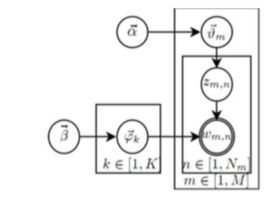
\includegraphics[height=3.7cm]{lda}
\end{center}

\subsection{Dirichlet分布与多项分布}
多项分布的共轭先验是Dirichlet分布,即若先验分布是Dirichlet分布,条件概率是多项分布,则按照贝叶斯公式后验概率与先验概率形式相同为了ichlet分布,具有良好性质,其中多项分布形式为:
\begin{displaymath}
p(x; n) = \frac{N!}{n_1! * n_2* ... *n_m!} x_1^{n_1} * x_2^{n_2} * ... * x_m^{n_m}
\end{displaymath}
Dirichlet分布:
\begin{displaymath}
p(x; n) = \frac{\Gamma(N)}{\Gamma(n_1) * \Gamma(n_2)* ... *\Gamma(n_m)} x_1^{n_1} * x_2^{n_2} * ... * x_m^{n_m}
\end{displaymath}
doc-topic, topic-word都是这样的Dirichlet-Multinomial共轭分布。

\subsection{Gibbs采样}
知道Gibbs采样。


\section{实现过程}
以下是实现具体细节,按实现时间排序。
\subsection{语料收集}
以下我们主要选取NIPS(Neural Information Processing Systems)2015作为本次的语料库。因为NIPS网站提供链接\cite{1},方便我们直接下载全部论文。

使用Python爬虫,从网页上找到所有论文的链接然后下载,因为NIPS网站排版具有一定格式(所有paper链接在一个<ul>标签中),我们先把这段HTML代码找出来,然后找出里面的url并下载对应文件。

\subsection{PDF数据处理}
由于我们得到的原始语料库是PDF文件,所以需要先提取里面的文本信息。一开始使用pyPdf直接提取文字,但是发现不能保留行内空格,如图:
\begin{center}
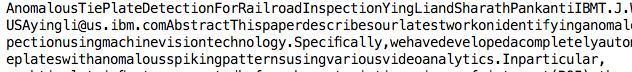
\includegraphics[width=13cm]{section3/1}
\end{center}

这时候我们有两种解决方案:
\begin{enumerate}
	\item	没有空格的英文分词
	\item	尝试另外个工具包
\end{enumerate}

后来我们使用一个叫作PDFMiner的Python工具包,通过判断PDF中两个字符之间的间隔大小来进行分词。
\begin{center}
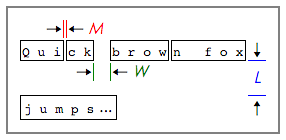
\includegraphics[height=3cm]{section3/2}

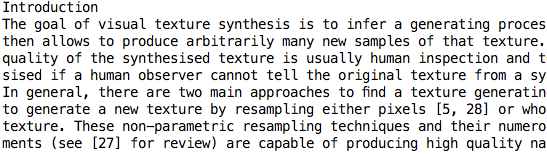
\includegraphics[width=13cm]{section3/3}
\end{center}

通过PDF转换成文本数据,我们也把论文中的图片和一些数学公式去掉了,剩下的基本是文字内容。

把数字和标点符号去掉,可以通过简单的正则表达式匹配完成。因为数字和标点对我们的topic model而言提供的信息量很少,所以这样处理十分合理。同时我们也统一转换成小写字母。因为LDA是一种\emph{词袋模型}(bag of words),最终只需要词频分布,所以我们不需要断句等工作。
\begin{center}
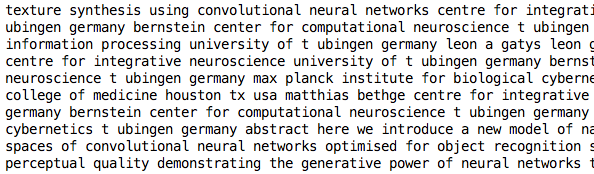
\includegraphics[width = 12cm]{section3/4}
\end{center}

相对中文而言,学术论文大多是用英文书写的,所以分词不是必须的。

文本提取后 \underline{部分}词频统计如图:
\begin{center}
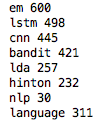
\includegraphics[height = 3.7cm]{section3/demo_word}
\end{center}

\subsection{单词筛选}
一个直觉的想法就是如果我们把在学术领域中没有特殊含义的词去掉以后,最终效果会有显著提升。

1.	回想在PDF转换到文本数据的过程中,我们可能引入了一些\textbf{噪声},如可能把公式中的字母也包含进来了,或因为我们的转换程序中间隔设置不合理有错误的单词提取结果。能否把这些"单词"去掉?如下例子中的的cid

\begin{center}
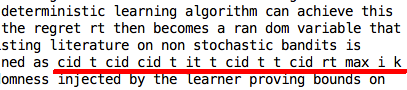
\includegraphics[height = 2cm]{section3/5}
\end{center}

针对以上问题,我\underline{根据单词长度进行筛选}
\begin{itemize}
	\item	单词小于等于2个字符,认为对于LDA没有特殊含义,直接去掉(去掉的单词包括a, I, am, be, he 还有德语de等)
	\item	单词长度大于15字符,认为是PDF转换结果出错,所以直接去掉。(剩下的PDF转换出错结果占比例较少)
\end{itemize}

2.	另外英文中普遍存在有禁用词(stop word)的情况,在这里我\underline{使用NLTK的} \underline{禁用词语料库进行处理}:
\begin{lstlisting}
	sw7 = stopwords.words('english')
	word_dict = [word for word in word_list if word not in sw7]
\end{lstlisting}

在文献领域也有领域的禁用词,如cid, reference, abstract, 针对这些词我建立了自己的禁用词表。

3.	英文与中文不同在于英文还有形式上的变化,为了让结果更准确,决定对词提取语干/词干。根据课本NLTK介绍,我们使用PorterStemmer作为我们词干提取器(参照了课本"规范化文本"一节)。
\begin{lstlisting}
	porter = nltk.PorterStemmer()
	word_dict = [porter.stem(word) for word in word_dict]
\end{lstlisting}

这里有一个问题,如关键词``R-CNN''(Region Convolutional Neural Network)会首先分成``R CNN''两个单词(去掉标点字符), 然后因为字母R长度为1,会被删去,剩下``CNN'',那么这样的结果是否合理?可以在后续研究中探讨。

\subsection{初步尝试LDA效果}
以上处理完以后,我们对每篇论文进行词频统计,并把结果存储为稀疏矩阵格式,使用lda类进行训练,结果如下(k=7,显示每个类别最可能生成的单词)

\begin{center}
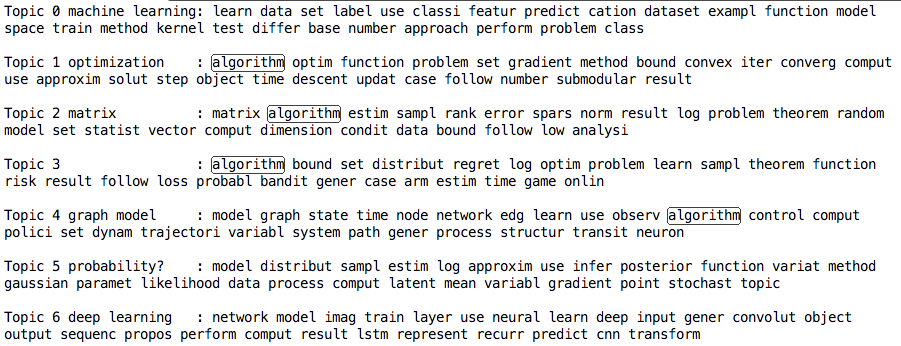
\includegraphics[width=13cm]{section3/result1}
\end{center}

我们发现,虽然``algorithm''这个单词在每个类别中排名都比较靠前,但是其实在文献语料库中普遍存在,所以对我们判断一篇文章的主题并没有太大帮助,考虑如何改进把这些词去掉?另外topic 3不知道是什么主题。

\subsection{改进1}
我首先的想法是给词频\textbf{设置一个区间},去掉频率出现过高的词和出现次数过少的词。

那么出现次数过少的词又是什么呢?有部分作者人名和提取文本失败的结果。考虑在一百万词中只出现1次,可能反而降低了LDA效果。所以对低频词也有阈值来筛选,\underline{去掉长尾}。\footnote{最后实验中我们使用的频率区间为(7, 4000)次。}

另外我们发现有两个字母的关键词,应该出现在我们的词典中,但是被筛走了,比如EM(代表expectation maximization算法)。所以我们又建立了一个小词典来加入这些之前处理中被排除的词。

\subsection{改进后效果}
详见后面``效果分析''
\subsection{More?}
以上结果看起来比较科学,但是毕竟是\emph{人手筛选过}的单词列表,不够自动化,于是进一步考虑能否让计算机自动计算哪些词对论文主题影响最大的呢?

根据我的分析,可以有两类不同的词筛选方法:
\begin{enumerate}
	\item	在NIPS2015中出现,\underline{但是一般英文文章中出现概率比较低}的词(如报纸,小说)。
	\item	在一篇文章中经常出现但是\underline{在整个语料库中分布不均衡}的词。
\end{enumerate}
以上是受到同学写的TF-IDF影评分析启发。

由于NLTK已自带语料库,所以我打算继续充分利用这个工具包。针对以上第一个思路,按两个语料库出现单词的词频之比来排序:
\begin{displaymath}
	\frac{p_{NIPS}}{\alpha + p_{others}}
\end{displaymath}
增加$\alpha$来平滑概率,因为专业名词如CNN,NLP在普通文章中不可能出现。
然后去掉比值较小的单词,以下是NIPS语料库和古腾堡语料库对比的结果,比值高代表在NIPS中更容易出现(方便起见使用频数之比代替频率之比):
\begin{center}
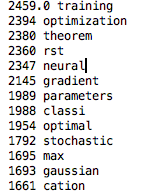
\includegraphics[height=4.0cm]{section3/high}
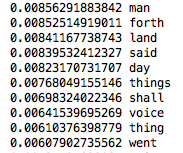
\includegraphics[height=4.0cm]{section3/low}
\end{center}
去掉比值小于1的单词后使用LDA结果发现结果基本不变,并且看起来已经比较合理,于是以下针对第2点的TF-IDF没有实现:
\begin{displaymath}
	p(x_i) * \mathrm{log} \frac{|D|}{\alpha + |D_i|}
\end{displaymath}

\section{效果及分析}
这里只给出最终程序的部分结果,更多中间结果和分析过程在上一节中提到,文中给出的图如果不够清晰可以打开附件中的原图片查看。
\subsection{How to Run It?}
To run my program, you may need to:
\begin{itemize}
	\item	Install Python2, NLTK, PDFMiner, lda
	\item	Download my source code
	\item	Download data from here\cite{2} to directory data/
	\item	Run preprocessing program in src/pre directory
	\item	Run src/gen to generate dict and input data of lda
	\item Run src/run.py to demostrate the lda model
\end{itemize}

\subsection{数据集效果}
在这次项目开发中,我们使用NIPS2015的论文作为语料库

\begin{center}
\begin{table}[!ht]
\centering
\caption{文章字数(word)统计}
\large
\begin{tabular}{|c|c|c|c|}
\hline
文章数 & 总单词数 & 筛选后的字数 & 平均每篇文章单词数\\
\hline
403 & 3229239 & 2148449 & 5331\\
\hline
\end{tabular}
\end{table}


\begin{table}[!ht]
\centering
\caption{字典(dictionary)统计}
\large
\begin{tabular}{|c|c|c|c|}
\hline
文章数 & 总字典 & 筛选后条目 & 每篇文章出现的不同词\\
\hline
403 & 30000以上 & 9956 - 10537 & 600-750\\
\hline
\end{tabular}
\end{table}
\end{center}

首先是使用NLTK对单词/词根频率统计结果(依次为频率排名前100,前300,前1000的词频曲线):
\begin{center}
	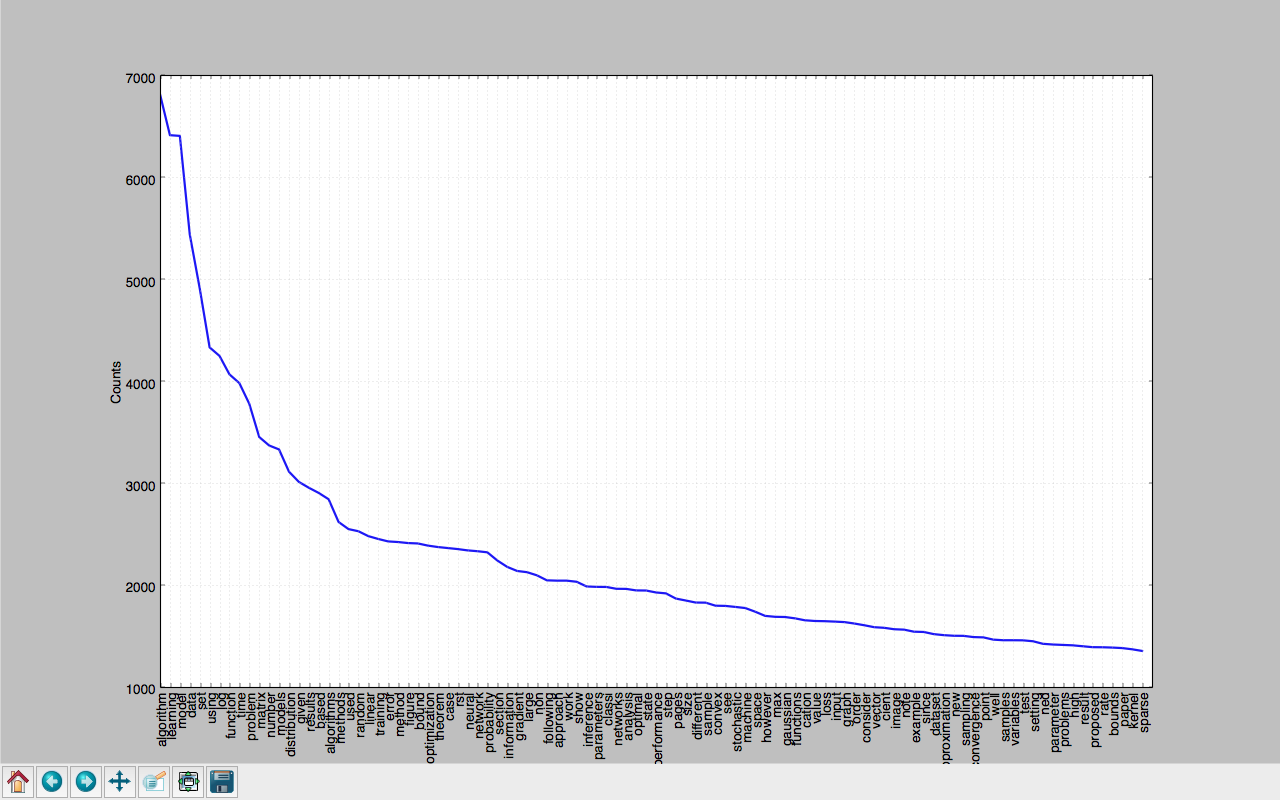
\includegraphics[height=6cm]{result/v1.0/dict-100}
	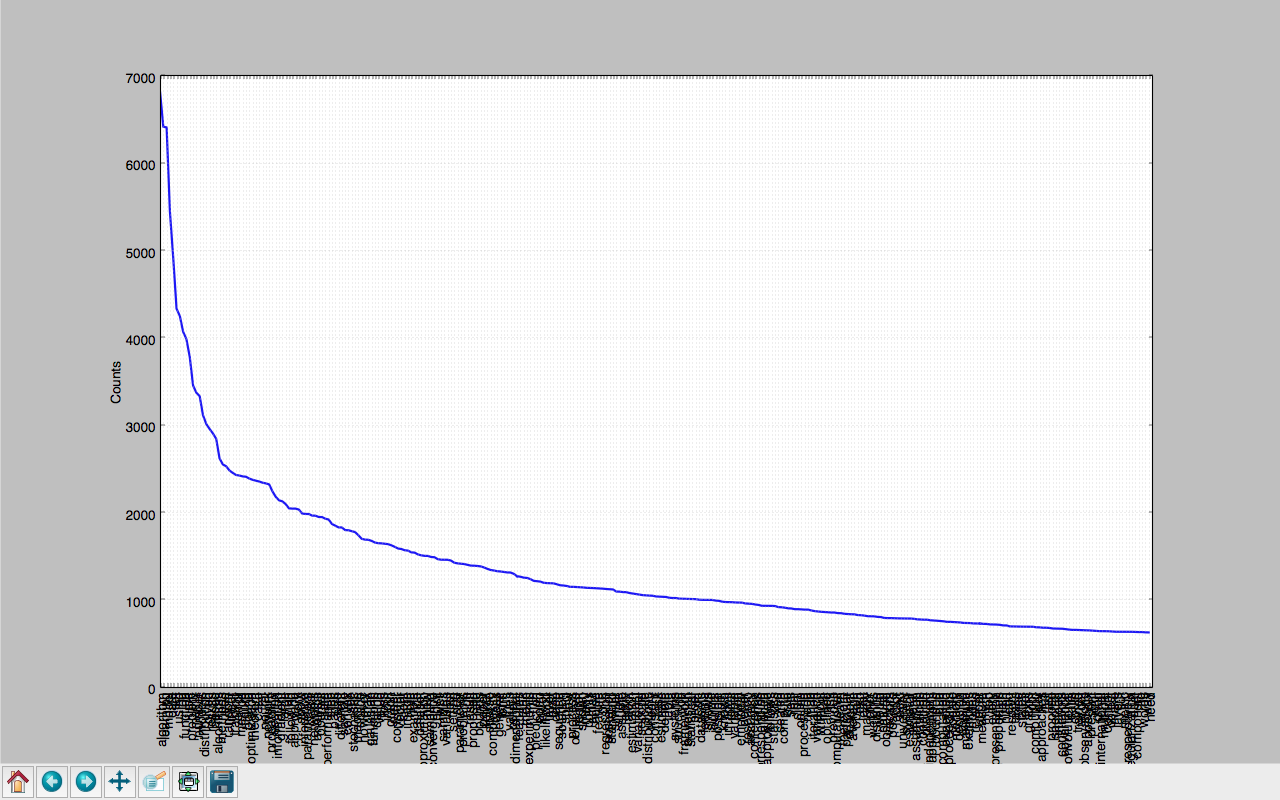
\includegraphics[height=6cm]{result/v1.0/dict-300}
	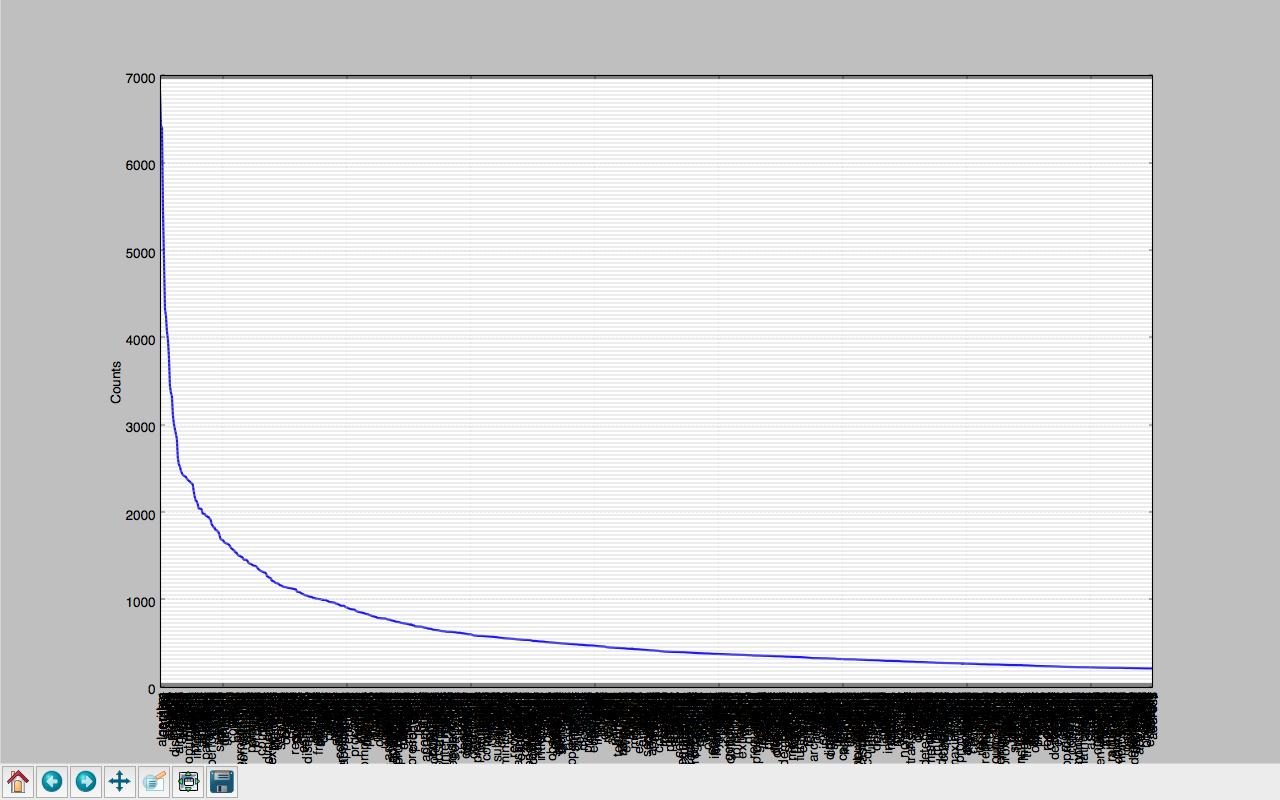
\includegraphics[height=6cm]{result/v1.0/dict-1000}
\end{center}
可以发现,排名与词频基本上是呈反比关系,一定层度上符合Zipf法则\cite{3}:
\begin{displaymath}
	f \propto \frac{1}{r}
\end{displaymath}
词干的频率曲线图与上面类似,但是在前100排名时,曲线形状不正常,如下图所示:
\begin{center}
	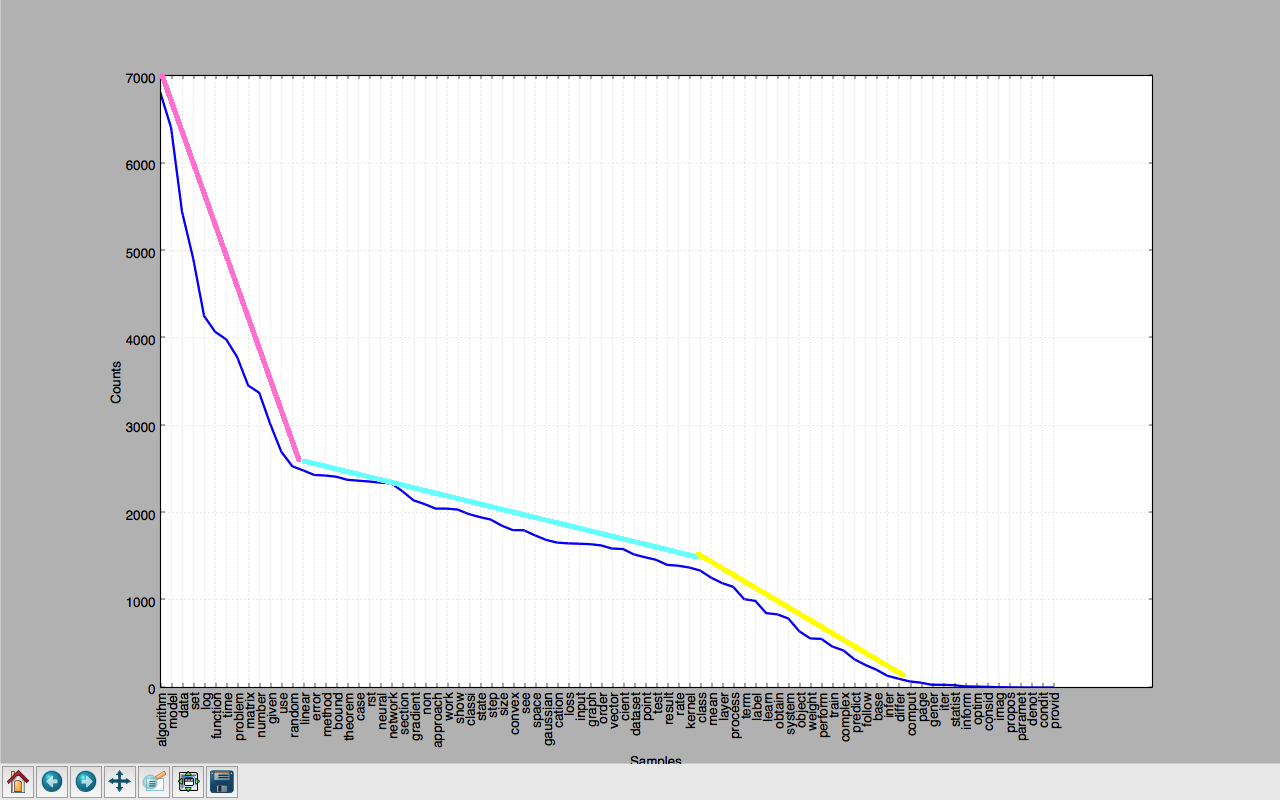
\includegraphics[height=6cm]{result/v1.0/stem-100}
	
	我们可以看到前100的词干频率曲线类似于三段分段直线。
	
	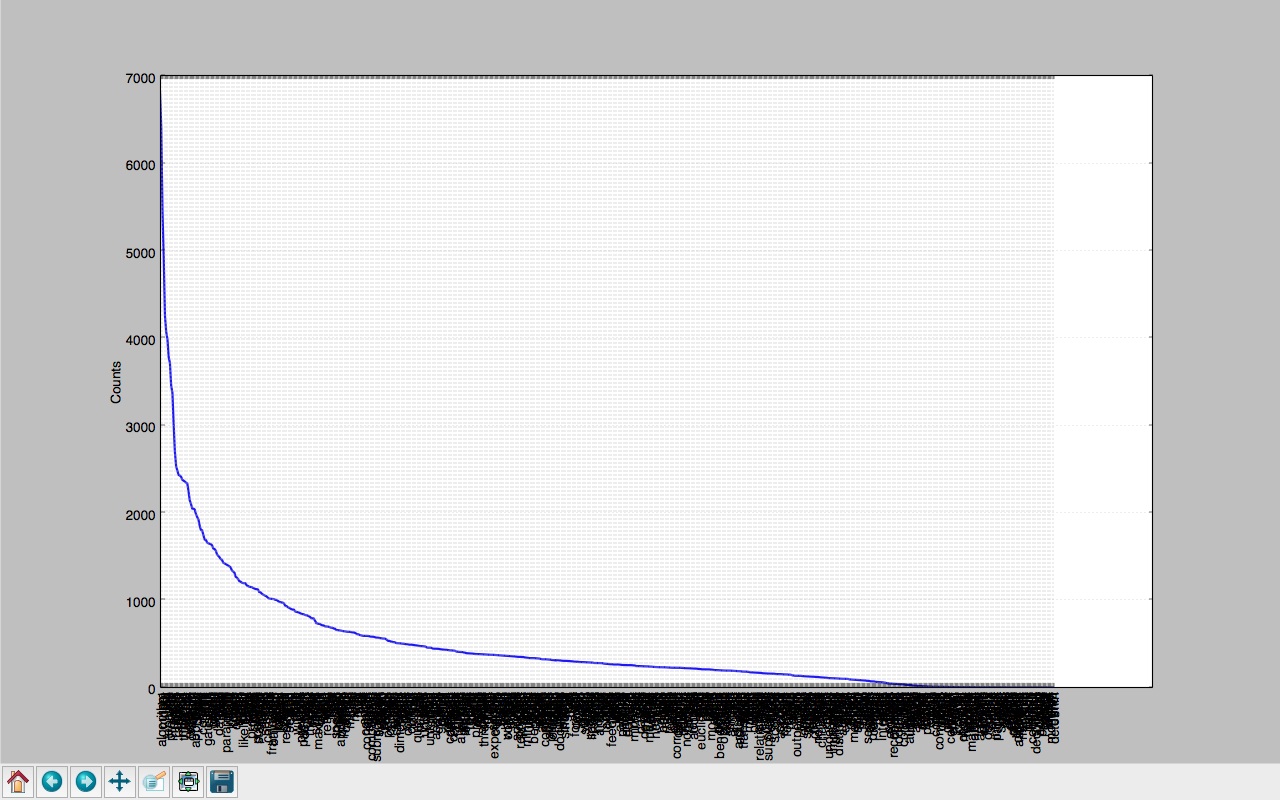
\includegraphics[height=6cm]{result/v1.0/stem-1000}
	
	而前1000的排名总体效果还是与双曲线接近。
\end{center}

\subsection{LDA主题效果}
Latent Dirichlet Allocation 训练时的log likelihood曲线如图,可以发现在迭代800-1000次以后已经收敛了(实验中一开始迭代了1500次,但是从效果上来看有over-fitting的嫌疑,后来只迭代了800次)
\begin{center}
	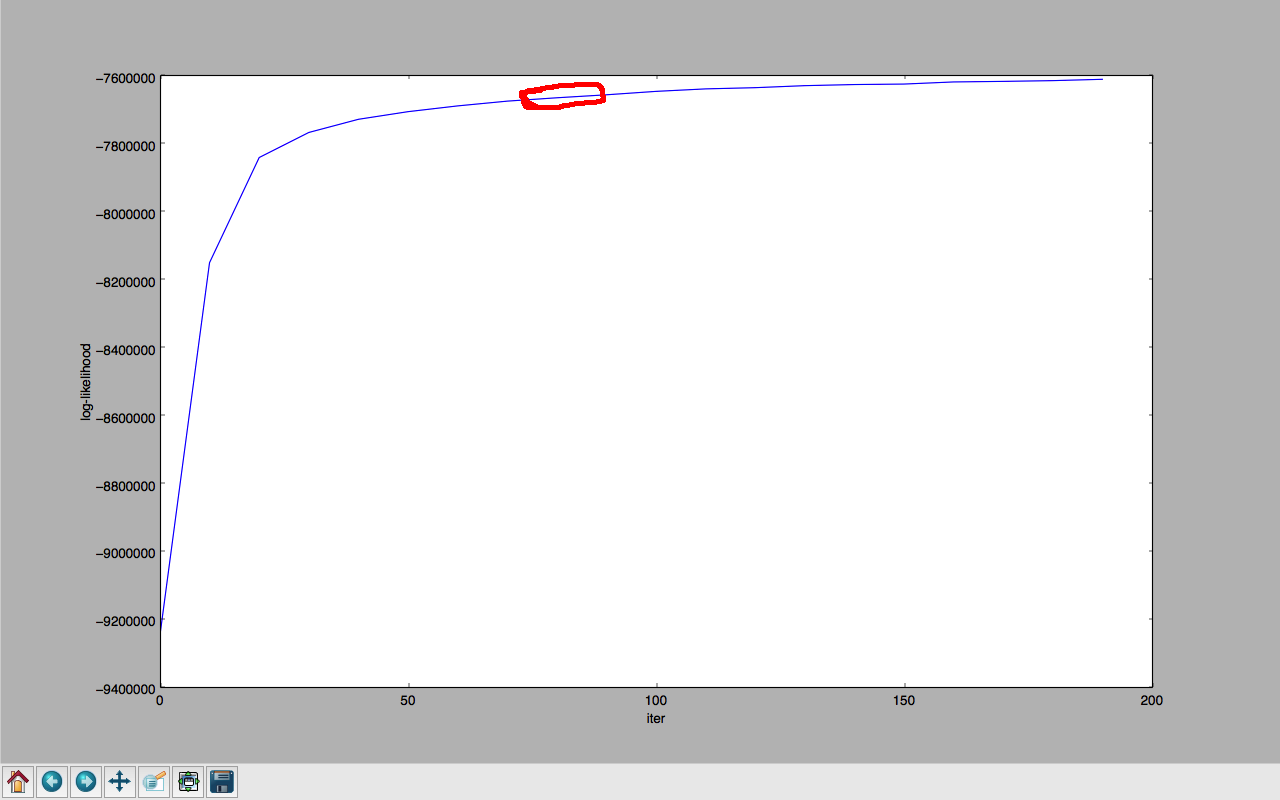
\includegraphics[height=6cm]{result/v2.0/lda-iteration}
\end{center}

\begin{center}
\begin{table}[!ht]
\centering
\caption{LDA运行情况}
\large
\begin{tabular}{|c|c|c|c|c|}
\hline
文章数 & 总字典 & 每篇文章出现的不同词 & topic &运行时间\\
\hline
403 & 9956 - 10537 & 600-750 & 7 & 138.58s\\
\hline
\end{tabular}
\end{table}
\end{center}


主题相关的词如下:
\begin{center}
	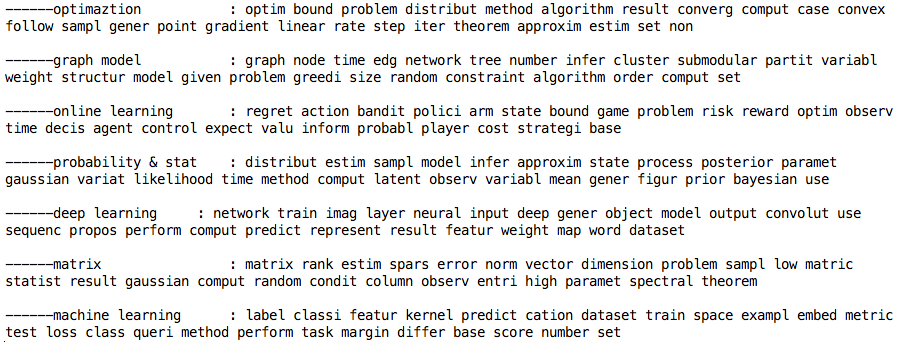
\includegraphics[width=15cm]{result/v2.0/result2}
\end{center}

归纳出来的主题(7个)分别是(0: optimization, 1: graph model, 2: online learning(bandit thing), 3: probability \& statistics, 4: deep learning, 5: matrix factorization, 6: machine learning)
,我们可以明显看到主题与对应词相关性。

Topic在语料库中的分布(每篇文章取概率最大的主题):
\begin{center}
	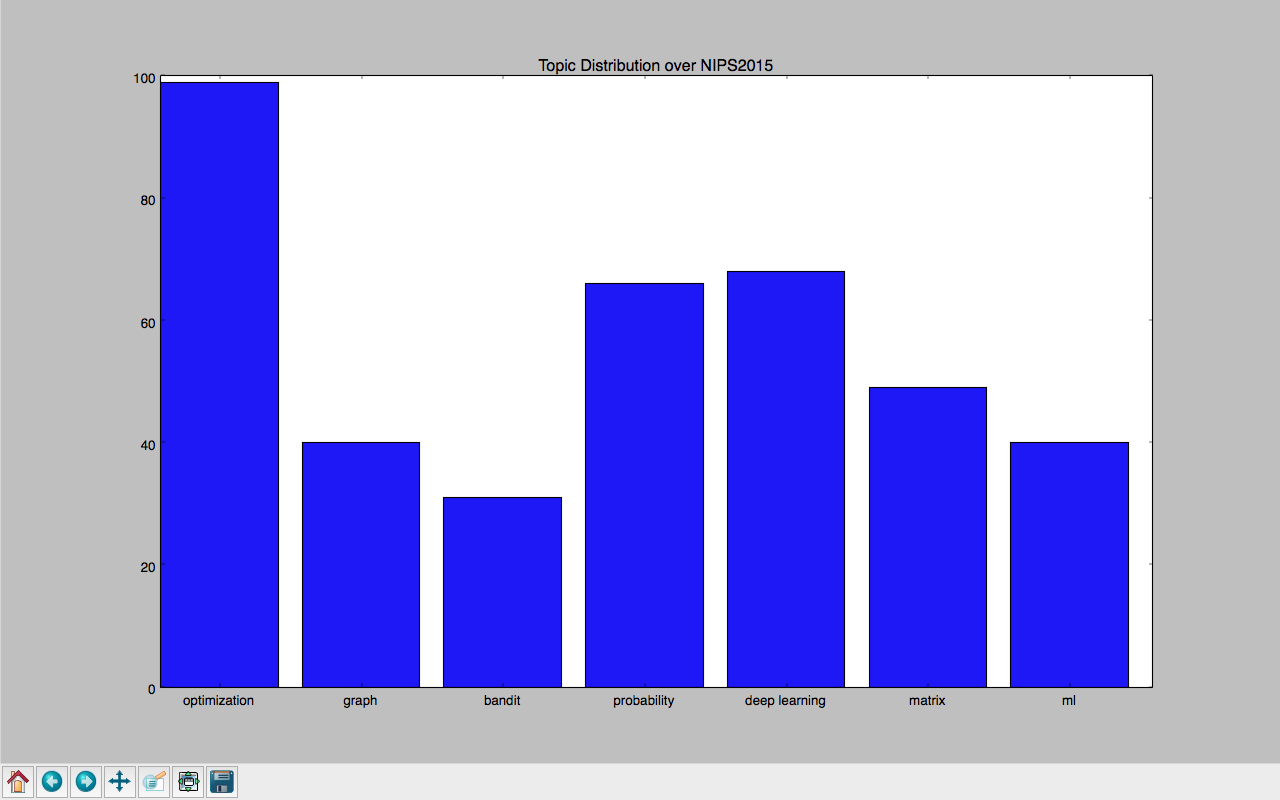
\includegraphics[width=10cm]{result/v2.0/topic-distribution}
\end{center}

我们发现第一类主题(优化)在语料库中出现的可能性最高,优化问题在机器学习的文献中普遍存在,所以这个主题中的词都是在语料库中常见的词,那么像这样\emph{有一个主题包含有全部常用词}的情况是否合理呢?回想起隐含Dirichlet分布的文本模型,先从doc-topic中抽取一个topic,然后按照topic-word分布生成词,如果一个主题把所有常用词都包含了,让别的主题更专注于更专业的词,可能最后产生的概率更大。

在训练LDA时我们使用9:1随机把文章分到训练集与测试集中,以下是在测试集上的LDA对单篇文章主题分类效果:
\begin{center}
	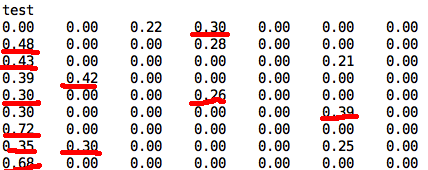
\includegraphics[width=10cm]{result/v2.0/single-doc}
\end{center}

另外我们发现一个topic的相关词有``Bandit'', ``arm''等,一开始不知道以为是算法出错了,结果上网搜索后发现是一种online learning的方法,主要应用在计算广告中,这也说明我们的系统真的起到了主题发现的作用,通过topic model而不是人眼浏览论文就能发现学术会议的几大主题,十分方便。

\section{The End}
到这里我们基本完成了本次``提取NIPS主题''的任务,以下是总结。
\subsection{总结}
在这次项目中我们实现了一个文献主题提取的系统,并更深入了解了LDA模型。LDA作为流行的topic model一种,在新闻自动分类,用户评论关键词提取,甚至个性化推荐中有重要应用。

另外,做到后面我清楚认识到主题离真正语义上的``研究方向''还是有一定距离的,topic主要把语义相近的词归为一个类别,如上面主题中的cnn, lstm虽然都属于深度学习,但是一个主要是图像处理,一个主要是语音和语言的处理,真正想要发现``研究方向''应该要区分这样的词到不同topic中去。

自然语言处理对我来说一直是一个比较繁琐的过程,在本次课程项目,我的时间主要花在获取数据和文本处理上面,可见有专人帮忙构造语料库可以节约大量时间。

这是我第一次没完全看懂算法就直接拿来用的项目,之前其他课程中我都是手写的(比如语音处理的MFCC,比如HMM),但是写一个project十分的慢。这个学期我们只有18周,到今天为止同学们已经连续忙碌考试和课程项目了超过一个月了,做完这个还有2个项目要完成。所以我想试一下用网上给出的机器学习工具包来减轻工作量(虽然文本处理也花了不少时间)。会用一个算法,远比了解算法原理细节要难,等完成所有项目后,打算在假期继续研究LDA原理\cite{6},目前知道Gibbs采样但是不知道在LDA中有什么用。

\subsection{Counterclaim?}
现在回顾项目实现过程中,发现有一些可以改进的地方:
\begin{itemize}
	\item	PDF转文本数据结果不应该这么差(在有些文章中还是不能把单词分开)。这是不应该出现的,因为如果手工对这些PDF文件进行选择-赋值-粘贴到.txt文件,总是有办法能分开的。
	\item	手工筛选词典不太科学,因为LDA就是要自动发现单词和主题之间的关系,应该一开始就只使用TF-IDF来过滤。
	\item	本来想用微软的lightlda(据说有很多优化,非常快,所以才想做LDA方面的project),但是始终配置安装不成功,最后使用的一个叫lda的Python模块,比较慢(400篇文章, 10000种单词,总共1,000,000词,7个主题,训练了138.58秒)。
	\item 因为字典大小(数据维数)始终在变,所以难以比较不同字典上使用的LDA模型,下次做项目应该使用相同大小的字典从而比较效果?
	\item	因为效果比较客观,训练比较慢,所以没有对不同主题数条件下的结果进行对比。
\end{itemize}

在即将完成本项目的时候,突然发现类似的方法已经有人做过了\cite{4}。对比一下提取出来的主题,发现大部分主题相同,但是有一类以``Bandit'', ``arm''等我认为是online learning的主题,但是网站上标成了theory。\\
~\\
总体来说我们实现的LDA是有效的。

\newpage
\section{Thank You}
\indent\indent 感谢您的仔细阅读!

Report generate in \LaTeX

View this project on GitHub\cite{5}

Full data used in this project is available here\cite{2}

高清大图可以查看其他附件。


\begin{thebibliography}{99}
\bibitem{1} \url{http://papers.nips.cc/book/advances-in-neural-information-processing-systems-27-2015}
\bibitem{2} \url{not availabie now}
\bibitem{3} Manning C D, Schutze H, et al. 统计自然语言处理基础[M]. 电子工业出版社, 2005.
\bibitem{4} \url{http://cs.stanford.edu/people/karpathy/nips2015/}
\bibitem{5} \url{https://github.com/kjkszpj/NlPS}
\bibitem{6} Steven Bird, Python自然语言处理.
\bibitem{7} LDA数学八卦
%todo课本
%todo lda-pdf
\end{thebibliography}

\end{document}